\documentclass[12pt]{article}

\usepackage[spanish]{babel}
\usepackage[utf8]{inputenc}
\usepackage{graphicx}
\usepackage{geometry}
\usepackage{xcolor}
\usepackage{fancyhdr}
\usepackage{lastpage}
\usepackage{pdfpages}
\usepackage{listings}
\usepackage{schemata}

\geometry{top=25mm,left=15mm,right=15mm,a4paper}

\pagestyle{fancy}
\fancyhf{}
\lhead{Analisis de Algoritmos}
\cfoot{Página \thepage\ de \pageref{LastPage}}

\graphicspath{./}

\begin{document}
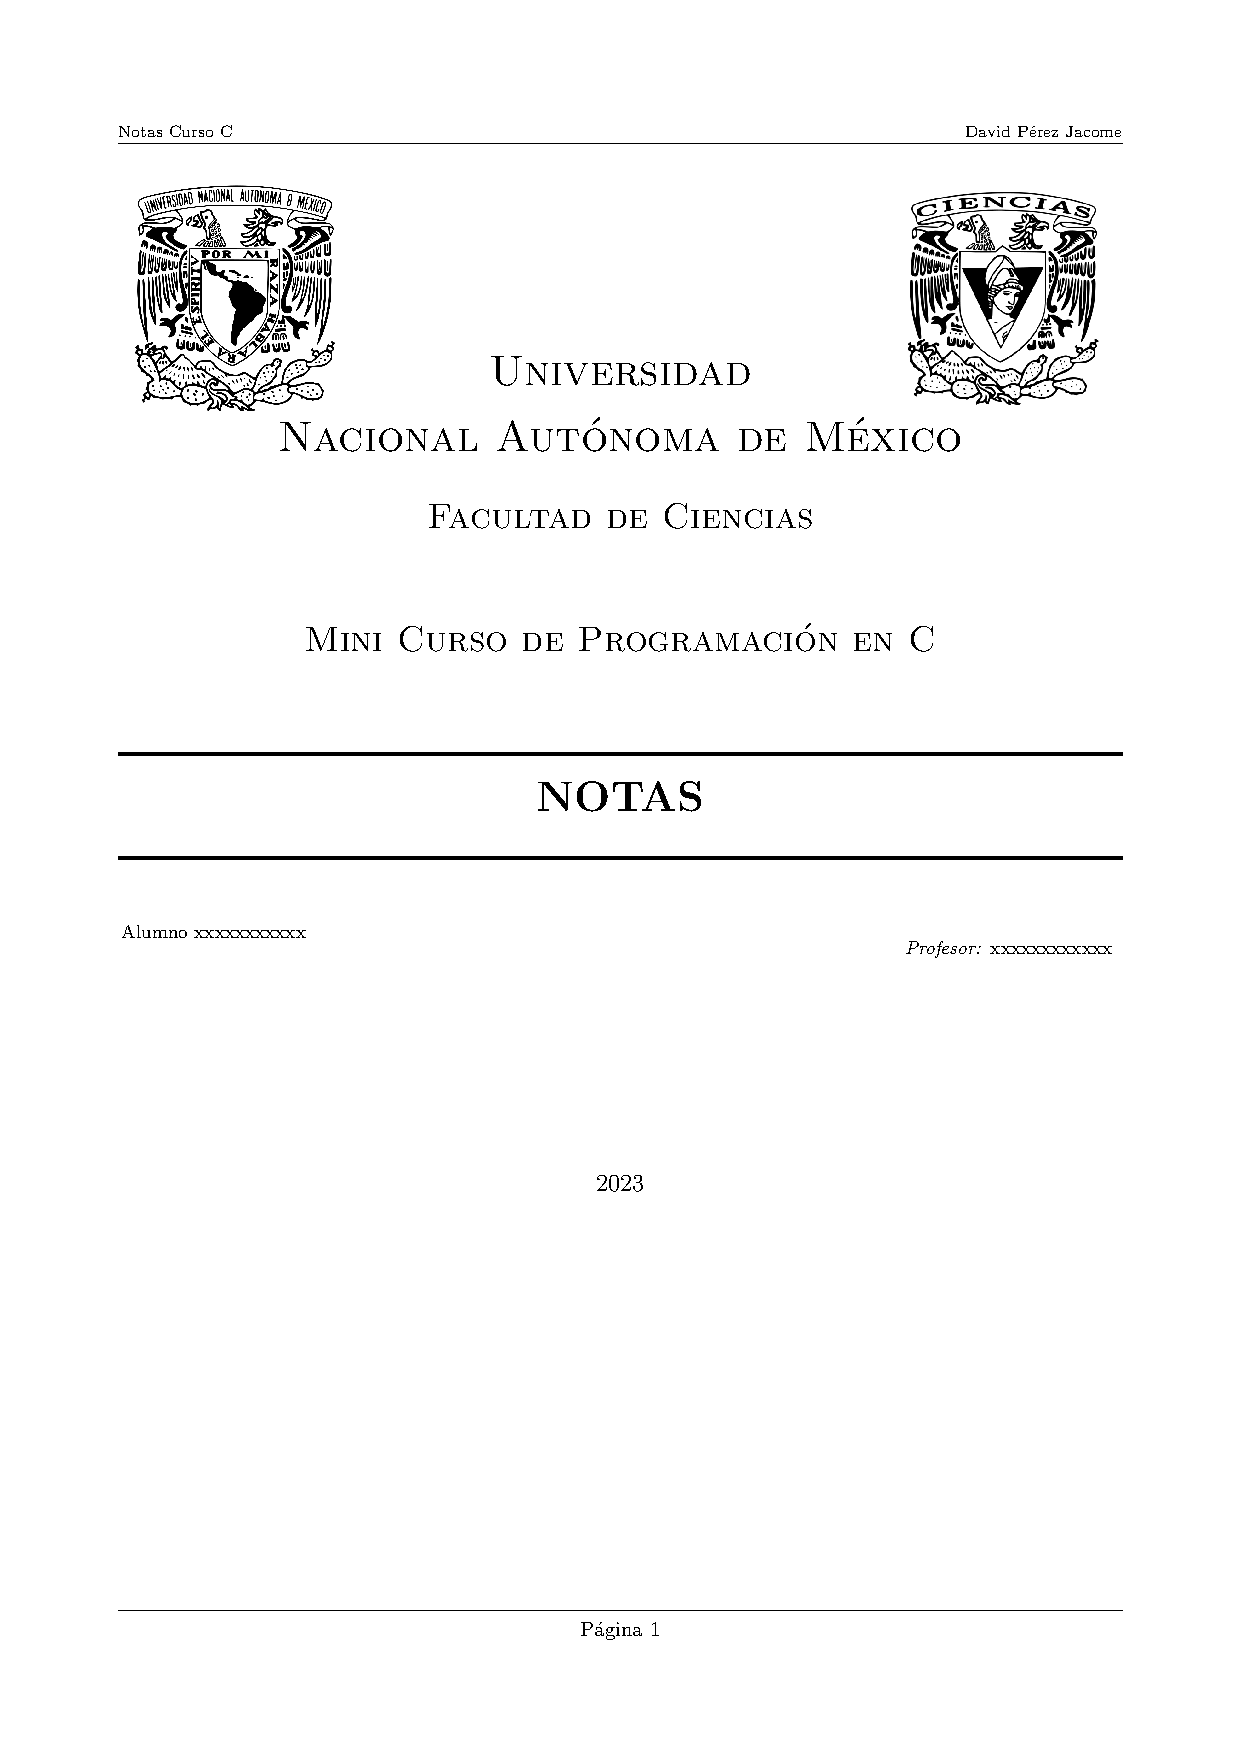
\includepdf{Portada.pdf}
{\color{blue} \section*{\textbf{Notas del Curso de Aprender a Programar con C.}}}
\vspace{1em}

{\color{red} \subsection*{\textbf{INTRODUCCIÓN.}}}

Inicialmente me di a la tarea de escribir este pequeño curso para futuras generaciones que  quieran aprender a programar y no sepan el como empezar, de igual 
manera es un pequeño repaso pasa fundamentar las bases de un buen curso, cabe recalcar que me guie de un curso en ingles de la plataforma \textbf{COURSERA} "Programming Fundamentals".\\

En este curso como lo describe perfectamente el titulo vamos a sembrar los fundamentos generales que nos van a servir para aprender a programar, como estudiante de Ciencias de la Computación tratare de ser lo más descriptivo y claro que me sea 
posible pero si en algún momento no es el caso y esta costando trabajo, me pueden contactar a traves de la dirección de correo electronico: \textbf{david1956@ciencias.unam.mx} y con gusto podre orientarlos en el contenido de este mini curso.\\
\\


{\color{red} \subsection*{\textbf{SEMANA 01.}}}


{\color{blue} \subsubsection*{\textbf{Programación: Planifica primero, luego codifica.}}}

Muchos programadores novatos intentan sumergirse directamente en la escritura del código (en el lenguaje de programación) como primer paso. Sin embargo, escribir el código en realidad es un paso mucho más tardío en el proceso. Un buen programador planificará primero y escribirá después, posiblemente dividiendo una tarea de programación grande en varias tareas más pequeñas en el proceso. 
Incluso cuando se les advierte que planeen primero y codifiquen después, muchos estudiantes de programación ignoran el consejo, después de todo, ¿por qué "perder" 30 minutos planeando cuando tienes poco tiempo debido a todo el trabajo que tienes que hacer? Sin embargo, este intercambio presenta una falsa economía: 30 minutos de planificación podrían ahorrar horas 
intentando que el código funcione correctamente. 
Un código bien planificado no solo es más probable que sea correcto (o al menos se acerque a la corrección), sino que también es más fácil de entender, y por lo tanto, de corregir.\\

Para tratar de entender mejor la importancia de planificar antes de escribir, imagina una analogía con la construcción de una casa o un rascacielos. 
Si te encargaran construir un rascacielos, ¿empezarías a construir de inmediato, descubriendo cómo está diseñado el edificio sobre la marcha? Esperemos que no. En su lugar, tú (o un arquitecto) diseñarías los planos del edificio primero. Estos planos se refinarían de forma iterativa hasta que cumplan con las especificaciones de todos: deben cumplir con los requisitos del propietario del edificio y ser factibles de construir. Una vez que se completen los planos, deben ser aprobados por el gobierno local. La construcción real solo comienza cuando los planes están completamente terminados. La programación debe hacerse de manera similar: primero se debe crear un plan completo (un algoritmo) y luego construirlo (implementarlo en código).\\

Dijimos que el corazón de la programación es descubrir cómo resolver una clase de problemas, no solo un problema en particular. 
Esta distinción se explica mejor con un ejemplo. Considera la tarea de determinar si un número en particular (por ejemplo, $7$) es primo. Con suficiente conocimiento de matemáticas (es decir, la definición de número primo y las reglas de división), se puede resolver este problema y determinar que $7$ es, de hecho, primo. 
Sin embargo, un problema de programación típicamente analiza una clase más general de problemas. Por lo general, no escribiríamos un programa para determinar si $7$ es primo, sino más bien un programa que, dado un número $N$, determine si $N$ es primo. Una vez que tenemos un algoritmo para esta clase general de problemas, podemos hacer que la computadora resuelva cualquier instancia particular del problema por nosotros.\\

Cuando examinamos una clase de problemas, tenemos parámetros que nos indican qué problema particular de la clase estamos resolviendo. 
En el ejemplo anterior, la clase de problemas está parametrizada por $N$, el número que queremos probar si es primo. Para desarrollar un algoritmo para esta clase de problemas, debemos tener en cuenta todos los posibles valores legales de los parámetros. Como veremos más adelante, los lenguajes de programación nos permiten restringir qué tipo de información puede representar un parámetro, para limitar los valores legales a aquellos que tienen 
sentido en el contexto del problema. Para la prueba de primalidad, querríamos que nuestro parámetro $N$ esté restringido de manera que solo pueda contener números enteros. No tendría sentido verificar si las letras, las palabras o los archivos son primos.\\

Para escribir un programa que tome cualquier número $N$ y determine si $N$ es primo, primero debemos idear el algoritmo para esta clase de problemas. Como dijimos antes, si abordamos el problema escribiendo código a ciegas, terminaremos con un desorden, al igual que construir un rascacielos sin un plan. Idear el algoritmo adecuado para una clase de problemas es una tarea desafiante y generalmente requiere un trabajo y una reflexión significativos.\\

{\color{blue} \subsubsection*{\textbf{Tecnica de los 7 pasos.}}}

\textbf{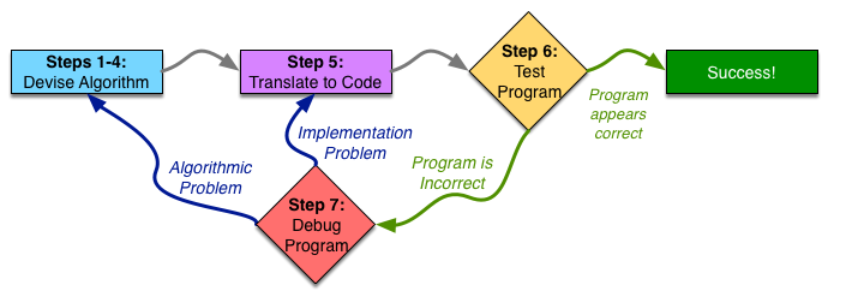
\includegraphics[scale = 0.55]{images/7 pasos.png}}\\

\begin{enumerate}
    \item 1-4 : Idear Algoritmo.
    \item 5: Traducir a codigo.
    \item 6: Probar programa.
    \item 7: Debuggear o coreegir errores o buggs
\end{enumerate}

{\color{blue} \subsubsection*{\textbf{Algoritmos}}}

Un algoritmo es un conjunto claro de pasos para resolver cualquier problema en una clase particular. Por lo general, los algoritmos tienen al menos un parámetro; sin embargo, existen algoritmos sin parámetros, simplemente están restringidos a un problema específico en lugar de una clase más general. Podemos discutir y pensar en algoritmos sin necesidad de tener un conocimiento particular de las computadoras; un buen algoritmo no solo puede ser traducido a código, sino que también podría ser ejecutado por una persona sin conocimientos específicos sobre el problema en cuestión.\\

Aunque las computadoras solo pueden trabajar con números, podemos imaginar algoritmos que podrían ser ejecutados por personas y que pueden trabajar con una variedad de cosas. Por ejemplo, podríamos escribir algoritmos que operen con objetos físicos como bloques de LEGO o alimentos. Aunque implementar tales cosas en una computadora sería difícil (necesitaríamos que la computadora controle un robot para interactuar con el mundo físico), siguen siendo instructivos, ya que los principios fundamentales de diseño algorítmico son los mismos.\\

La computadora no "sabe lo que quieres decir" cuando escribes algo vago, ni puede deducir un "etc.". En cambio, debes ser capaz de describir exactamente lo que deseas hacer paso a paso. Describir con precisión los pasos exactos para realizar una tarea específica es un poco complicado, ya que estamos acostumbrados a que las personas comprendan implícitamente los detalles que omitimos. La computadora no lo hará por ti (en ningún lenguaje de programación).\\

\begin{enumerate}
    \item PASO 1: Elegir un parametro, valores y trabajarlo a mano.
    \item PASO 2: Idear las instrucciones para trabajar los valors del P1, Que se hizo para resolver el problema.
    \item PASO 3: Generalizar los pasos, encontrar el patron general (de particular a general).
    \item PASO 4: Prueba el algoritmo y garantizar que funciona con distintos valores. 
\end{enumerate}








\end{document}